\documentclass{article}
\usepackage{tikz}
\usetikzlibrary{positioning}

\begin{document}

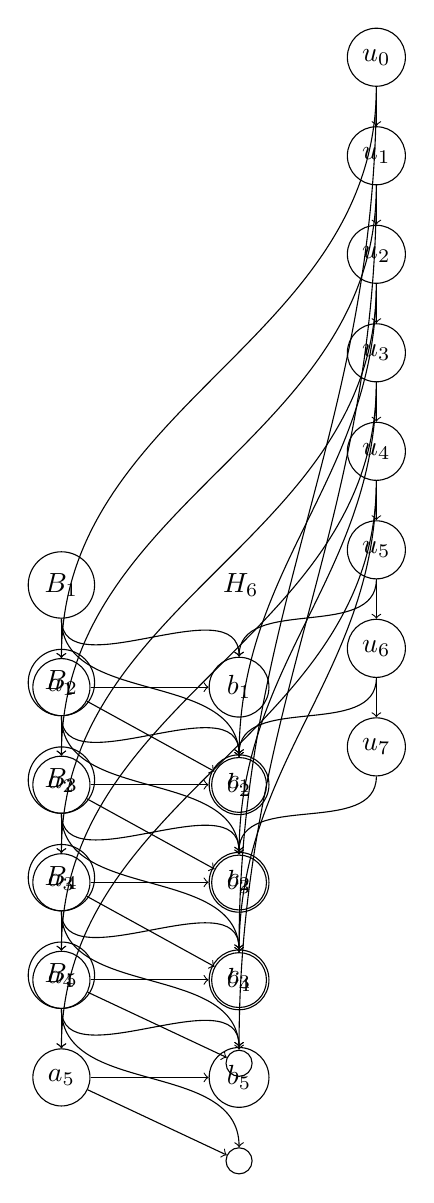
\begin{tikzpicture}[node distance=0.5cm and 1.5cm]
    % Define nodes for the top part of the graph
    \node[circle,draw] (u0) at (0,6) {$u_0$};
    \node[circle,draw] (u1) [below=of u0] {$u_1$};
    \node[circle,draw] (u2) [below=of u1] {$u_2$};
    \node[circle,draw] (u3) [below=of u2] {$u_3$};
    \node[circle,draw] (u4) [below=of u3] {$u_4$};
    \node[circle,draw] (u5) [below=of u4] {$u_5$};
    \node[circle,draw] (u6) [below=of u5] {$u_6$};
    \node[circle,draw] (u7) [below=of u6] {$u_7$};

    % Draw edges between the top part nodes
    \draw[->] (u0) -- (u1);
    \draw[->] (u1) -- (u2);
    \draw[->] (u2) -- (u3);
    \draw[->] (u3) -- (u4);
    \draw[->] (u4) -- (u5);
    \draw[->] (u5) -- (u6);
    \draw[->] (u6) -- (u7);

    % Define nodes for the bottom part of the graph
    \node[circle,draw] (a1) at (-4,-2) {$a_1$};
    \node[circle,draw] (b1) [right=of a1] {$b_1$};
    \node[circle,draw] (c1) [below=of b1] {$c_1$};
    \node[circle,draw] (a2) [below=of a1] {$a_2$};
    \node[circle,draw] (b2) [right=of a2] {$b_2$};
    \node[circle,draw] (c2) [below=of b2] {$c_2$};
    \node[circle,draw] (a3) [below=of a2] {$a_3$};
    \node[circle,draw] (b3) [right=of a3] {$b_3$};
    \node[circle,draw] (c3) [below=of b3] {$c_3$};
    \node[circle,draw] (a4) [below=of a3] {$a_4$};
    \node[circle,draw] (b4) [right=of a4] {$b_4$};
    \node[circle,draw] (c4) [below=of b4] {};
    \node[circle,draw] (a5) [below=of a4] {$a_5$};
    \node[circle,draw] (b5) [right=of a5] {$b_5$};
    \node[circle,draw] (c5) [below=of b5] {};

    % Draw edges between the bottom part nodes
    \draw[->] (a1) -- (b1);
    \draw[->] (a1) -- (c1);
    \draw[->] (a2) -- (b2);
    \draw[->] (a2) -- (c2);
    \draw[->] (a3) -- (b3);
    \draw[->] (a3) -- (c3);
    \draw[->] (a4) -- (b4);
    \draw[->] (a4) -- (c4);
    \draw[->] (a5) -- (b5);
    \draw[->] (a5) -- (c5);

    % Draw edges connecting the top and bottom parts
    \draw[->] (u0) to[out=-90,in=90] (a1);
    \draw[->] (u1) to[out=-90,in=90] (a2);
    \draw[->] (u2) to[out=-90,in=90] (a3);
    \draw[->] (u3) to[out=-90,in=90] (a4);
    \draw[->] (u4) to[out=-90,in=90] (a5);
    \draw[->] (u5) to[out=-90,in=90] (b1);
    \draw[->] (u6) to[out=-90,in=90] (b2);
    \draw[->] (u7) to[out=-90,in=90] (b3);
    \draw[->] (u0) to[out=-90,in=90] (b4);
    \draw[->] (u1) to[out=-90,in=90] (b5);
    \draw[->] (u2) to[out=-90,in=90] (c1);
    \draw[->] (u3) to[out=-90,in=90] (c2);
    \draw[->] (u4) to[out=-90,in=90] (c3);

    % Define nodes for the middle part of the graph
    \node[circle,draw] (B1) [above=of a1] {$B_1$};
    \node[circle,draw] (B2) [above=of a2] {$B_2$};
    \node[circle,draw] (B3) [above=of a3] {$B_3$};
    \node[circle,draw] (B4) [above=of a4] {$B_4$};
    \node[circle,draw] (B5) [above=of a5] {$B_5$};

    % Draw edges between the middle and bottom parts
    \draw[->] (B1) to[out=-90,in=90] (a1);
    \draw[->] (B1) to[out=-90,in=90] (b1);
    \draw[->] (B1) to[out=-90,in=90] (c1);
    \draw[->] (B2) to[out=-90,in=90] (a2);
    \draw[->] (B2) to[out=-90,in=90] (b2);
    \draw[->] (B2) to[out=-90,in=90] (c2);
    \draw[->] (B3) to[out=-90,in=90] (a3);
    \draw[->] (B3) to[out=-90,in=90] (b3);
    \draw[->] (B3) to[out=-90,in=90] (c3);
    \draw[->] (B4) to[out=-90,in=90] (a4);
    \draw[->] (B4) to[out=-90,in=90] (b4);
    \draw[->] (B4) to[out=-90,in=90] (c4);
    \draw[->] (B5) to[out=-90,in=90] (a5);
    \draw[->] (B5) to[out=-90,in=90] (b5);
    \draw[->] (B5) to[out=-90,in=90] (c5);

    % Label the middle part
    \node[right=of B1] {$H_6$};
\end{tikzpicture}

\end{document}